\chapter{Bootloader}

If you are stil here... buckle up. In this chapter we will familiarize ourselves with some concepts necessary to understand bootloaders
and then start writting our own.

Before we start it should be made clear that everything below applies to the Intel i-386 processor architecture (32-bit x86).
However, transferring that knowledge to different architectures should not be that difficult

\section{CPU Operating Modes}

When the computer turns on the x86 processor is automatically in \textbf{Real Mode}, which has some significant limitations. However,
it is kept even in newer processors for backwards compatibility reasons. 

When in Real Mode the CPU is running by default in 16-bit mode. While 32-bit registers are technically still available they 
should not be used, except when changing to Protected Mode (32-bit mode).

Another limitation of Real Mode is that you only have access to a specific size of memory. When referring to a memory 
address in Real Mode we use a 20-bit physical addressing. The Physical Address is referred to using a Segment and Offset like this: 
\[
\textbf{PA = Segment} \cdot \textbf{16 + Offset}
\]
Essentially, using this convention you can only represent a number if it can fit in a 5 digit hex. It is also apparent that
there are multiple ways to represent the same address. For example the physical address 0x12345 can be represented 
by 0x1234 and 0x0005, 0x1230 and 0x0045, 0x1200 and 0x0345... and so on. This way of addressing memory limits us to just 
below 1MiB of memory.

By now it should be clear that the addresses used in Real Mode are the actual physical addresses. This hinders us from protecting
memory and defining its owenership because every process can simply access all memory segments. We will get into virtual memory 
later on this book but I will give a brief explaination of how it helps with owenership just to clarify why physical 
addresses are limiting.

When having virtual addresses, our Operating System is responsible of mapping every virtual address to a physical onen.
When this mappning is done, the operating systems ensures that each program has its own range of physical addresses.
When two programs refer to the same virtual memory, very little does it matter, since the mapping will make sure they 
will refer to totally different physical addresses, rendering both unable to access eachothers' memory.

Having said that, Real Mode is simply inadequate for modern systems. This is why engineers came up with another CPU 
Operation Mode called \textbf{Protected Mode}. In this mode, while we still do not have any virtualization, we can 
take advantage of how memory is segmented to protect critical data from the user. This can happen by defining different 
memory segments with different privileges (ring levels) and letting the CPU decide if a piece of code has the privilages 
it tries to claim. This is decided according to the segment through which we are accessing that memory (we will se that in
practice). Memory management and CPU Operating Modes will have chapters of their own later in this book so we will not 
elaborate any longer here. For now let's focus on what a bootloader is and what it needs to do in its short but 
critical lifespan. 

\section{The Role Of The Bootloader}

When the computer turns on the first program to take control is the BIOS. Among other things, the BIOS transfers control to 
the bootloader which is then responsible for loading the OS. Modern systems use UEFI but in the sake of simplicity we 
will focus on BIOS.

First, the BIOS scans the data storage devices. More precisely it checks the first 512 bytes of each one, namely the Master Boot Record 
(MBR), which is the place a bootloader conventionally resides upon. If the last two bytes of the MBR are the word 0xAA55 the BIOS 
classifies the storage device as a bootable device.

Once the bootable is identified the BIOS loads the bootloader from the MBR to the memory address 0x7C00. This address has been
traditionally used by BIOS software to load the bootloader. Bootloader developers conventionally assume this is where their 
bootloader will is be loaded. The address 0x7C00 is way below the 1MiB accessible range and still leaves space below 
it for interrupt vectors (we will talk about them later).

After control has been passed to the bootloader it is now its job to load the rest of the operating systems. In later section we will 
discuss some techniques to overcome the 512-byte barrier and the limitations of the Real Mode. For now let's take a look in how
we can load the kernel.

\section{Loading The Kernel}

Let's start by dumping some code. Please do not be overwhelmed by it as we will explain it thoroughly shortly after.

\begin{lstlisting}[caption={Simple bootloader start in assembly}]
[ORG 0x7C00] ; This is where the bootloader is loaded in memory
[BITS 16]    ; Bootloader code starts in 16-bit mode

start:
    cli
    mov ax, 0x0700
    mov ss, ax       ; Set stack segment to 0x0700
    mov sp, 0x0000   ; Set stack pointer below of bootloader
    xor ax, ax       ; Zero-out ax
    mov ds, ax       ; Set data segment to 0
    mov es, ax       ; Set extra segment to 0

    mov ah, 0x02
    mov al, 1        ; Number of sectors
    mov ch, 0
    mov cl, 2
    mov dh, 0
    mov dl, 0x80
    mov bx, 0x1000    ; Segment
    mov es, bx
    xor bx, bx        ; Offset
    int 0x13
\end{lstlisting}
    
Let's analyze this line by line. 

First of all \texttt{cli} is used to prevent the system from triggering interrupts.
Since we have not dealt with setting up interrupt handling yet, they will just cause problems.

In lines 6 to 8 we are setting up a simple stack for our Real Mode. To understand these lines we must
remember how we address physical memory in Real Mode. It our Stack Segment pointer (ss) we choose segment \texttt{0x0700}
and in our Stack Pointer (sp) we define the offset \texttt{0x0000}. Now the physical address is calculated as such:
\[
\textbf{PA = 0x0700} \cdot \textbf{16 + 0x0000}
\textbf{ => PA = 0x7000 + 0x0000}
\textbf{    => PA = 0X7000}
\]
This address is chosen to be more than 512 bytes below \texttt{0x7C00}, the range where out bootloader is placed.
As mentioned, there are other combinations that could address the same memory as well.
Note that the bootloader might still run without lines 6 to 11, however, without having the stack set up
and the ax, ds and es registers zeroed-out the environment would be highly unpredictable.

Now that we are in a controllable environment we can load our kernel into memory. To do this we will must use
a very useful feature of BIOS, BIOS interrupts. Since we have not explained interrupts yet, we can think of them
as favors. More specifically when we trigger a BIOS interrupt we stop the execution of anything else, as the name states,
and have BIOS do what we ask. In this occasion by calling \texttt{int 0x13} we ask the BIOS to load some data from our
hard drive into our memory. However, before triggering the interrupt we must pass some parameters using some registers to 
tell BIOS exactly what it should do.

\begin{table}[h]
    \centering
    \begin{tabular}{|c|p{5cm}|p{4cm}|}
    \hline
    \textbf{Register} & \textbf{Purpose} & \textbf{Value Used} \\ \hline
    \texttt{AH} & BIOS function number & \texttt{0x02} (read sectors) \\ \hline
    \texttt{AL} & Number of sectors to read & \texttt{1} sectors \\ \hline
    \texttt{CH} & Cylinder number (part 1) & \texttt{0} \\ \hline
    \texttt{CL} & Sector number (bits 0–5) and high bits of cylinder (bits 6–7) & \texttt{2} (start at sector 2) \\ \hline
    \texttt{DH} & Head number & \texttt{0} \\ \hline
    \texttt{DL} & Drive number & \texttt{0x80} (first hard drive) \\ \hline
    \texttt{ES:BX} & Memory segment:offset where data is stored & \texttt{0x1000:0x0000} (i.e., \texttt{0x10000}) \\ \hline
    \end{tabular}
    \caption{INT 0x13, AH=0x02 — Disk Read BIOS Call Parameters}
    \label{tab:disk_read_params}
\end{table}
    
Since interrupt \texttt{0x13} provides multiple storage device related function we can use the \texttt{ah} register
to choose the \texttt{Read Sectors From Drive} function.
In the \texttt{al} register we can define the number of sectors (512-byte unit) we want to read. For simplicity
we will initially be reading just one.

Before understanding what registers \texttt{ch}, \texttt{cl} and \texttt{dl} we need to introduce a new addressing
model called \textbf{Cylinder-Head-Sector} (or CHS). As the name states, this model mirrors the concept of physical 
cylinders, heads and sectors a traditional hard drive uses. 

\begin{figure}[H]
    \centering
    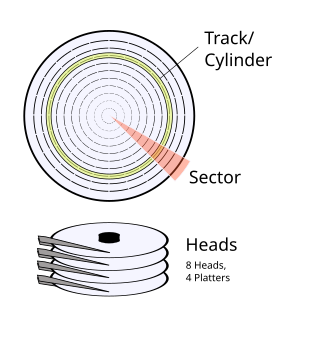
\includegraphics[width=0.4\textwidth]{images/chs_diagram.png}
    \caption{CHS addressing layout: cylinders, heads, and sectors}
    \label{fig:chs}
\end{figure}

As shown above, hard drives are constituted of platters which are essentially circular disks. On both surfaces
of these platters - both the top and bottom - data can be written magnetically by a device called head. So for 
4 platters we have 8 heads. 

Now imagine multiple cylinders with centers aligned with the platters'. The intersection of a platter's surface 
and a cylinder is called a track. Naturally we have \(\textbf{Cylinders} \cdot \textbf{Platters} \cdot \textbf{2}\)
number of tracks. Each track can be accessed by only one head.

Each track is divided into sectors, which we can visualize as circular sectors. Each sector is the smallest addressable
unit and has a size of 512 bytes.

When writting data to a hard drive we must specify the cylinder, the head and the sector along the track defined by the
cylinder and the head's surface. Each combination of CHS maps to a 512-byte unit or more precisely a Logical Block 
Address (LBA). First, we write data in cylinder 0, head 0, and sector 1 (sectors start counting from number 1). As we 
fill in sectors until sector 63 we can start filling up heads. When head 255 is filled, we fill in cylinder. The 
last available cylinder is 1023. 

\begin{itemize}
    \item \textbf{1024}: Cylinders (0–1023, 10 bits)
    \item \textbf{256}: Heads (0–255, 8 bits)
    \item \textbf{63}: Sectors (1–63, 6 bits), \textit{1-based indexing}
    \item \textbf{512}: Bytes per sector
\end{itemize}
  
Since CHS is limited at addressing 8.4 GiB of data it has been declared obsolete and replaced by direct LBA addressing.
However, the BIOS still offers this function.

Also, note that modern hard drives do not expose their geometrical structure and instead use an emulation layer for
CHS addressing.

For our case, since the first sector contains the bootloader, we want to start loading from sector number 2.
So we can set our cylinder to 0, our head to 0 and our sector to 2. Be careful when addressing cylinders
as their 2 high bits are defined in bits 6 and 7 of \texttt{cl}.

In the register \texttt{dl} we must specify the storage unit which we want to read data from.
Options \texttt{0x00} to \texttt{0x7F} correspond to floppy dics, while options \texttt{0x80} and higher
correspond to hard drives.

In registers \texttt{es:bx} we use the segment:offset addressing method to specify where in memory we want
to store the data we read.

\begin{lstlisting}[caption={Assembly to load the kernel}]
    mov ah, 0x02
    mov al, 1        ; Number of sectors
    mov ch, 0
    mov cl, 2
    mov dh, 0
    mov dl, 0x80
    mov bx, 0x1000    ; Segment
    mov es, bx
    xor bx, bx        ; Offset
    int 0x13
\end{lstlisting}

Finally, after having specified our parameters we can call \texttt{int 0x13} and let the BIOS do its job.